\documentclass[dvipdfmx,uplatex,oneside]{jsbook}
% %% fixes to LaTeX2e
% \usepackage{fix-cm}[2006/09/13 v1.1m]
% \usepackage{fixltx2e}[2006/09/13 v1.1m]

\usepackage[deluxe,uplatex]{otf}
\usepackage[T1]{fontenc}\usepackage{textcomp}%T1/TS1
% \usepackage{lmodern}
\usepackage[dvipdfmx]{graphicx}
\usepackage[dvipdfmx,table]{xcolor}%requires colortbl, array
\usepackage{framed}
\usepackage{wrapfig}
\definecolor{shadecolor}{gray}{0.9}
\definecolor{shadecolorb}{gray}{0.1}
\definecolor{reviewgreen}{rgb}{0,0.4,0}
\definecolor{reviewblue}{rgb}{0.2,0.2,0.4}
\definecolor{reviewred}{rgb}{0.7,0,0}
\definecolor{reviewdarkred}{rgb}{0.3,0,0}
\usepackage[utf8]{inputenc}
\usepackage{ascmac}
\usepackage{float}
\usepackage{alltt}
\usepackage{amsmath}

%% if you use @<u>{} (underline), use jumoline.sty
\IfFileExists{jumoline.sty}{
\usepackage{jumoline}
}

\newenvironment{shadedb}{%
  \def\FrameCommand{\fboxsep=\FrameSep \colorbox{shadecolorb}}%
  \MakeFramed {\FrameRestore}}%
 {\endMakeFramed}

\usepackage[top=10zw,bottom=12zw,left=10zw,right=10zw]{geometry}
%\usepackage[top=5zw,bottom=5zw,left=1zw,right=1zw]{geometry}

\newcommand{\parasep}{\vspace*{3zh}}
\setlength{\footskip}{30pt}

%% Bookmarkの文字化け対策(日本語向け)
\usepackage[dvipdfmx,bookmarks=true,bookmarksnumbered=true,colorlinks=true,%
     pdftitle={Qiita と Re:VIEW を使ってオンラインで記事を寄せあい同人誌を作って 同時にWebコンテンツとして公開できるシステムがこんなに便利なわけはない},%
     pdfauthor={日本Androidの会秋葉原支部ロボット部}]{hyperref}
\usepackage[dvipdfmx]{pxjahyper}



\newenvironment{reviewimage}{%
  \begin{figure}[H]
    \begin{center}}{%
    \end{center}
  \end{figure}}

\newenvironment{reviewdummyimage}{%
  \begin{figure}[H]
    \begin{center}\begin{alltt}}{%
    \end{alltt}\end{center}
  \end{figure}}

\newenvironment{reviewemlist}{%
  \medskip\small\begin{shaded}\setlength{\baselineskip}{1.3zw}\begin{alltt}}{%
  \end{alltt}\end{shaded}}

\newenvironment{reviewlist}{%
  \begin{shaded}\small\setlength{\baselineskip}{1.3zw}\begin{alltt}}{%
  \end{alltt}\end{shaded}\par\vspace*{0.5zw}}

\newenvironment{reviewsource}{%
  \begin{shaded}\small\setlength{\baselineskip}{1.3zw}\begin{alltt}}{%
  \end{alltt}\end{shaded}\par\vspace*{0.5zw}}

\newenvironment{reviewcmd}{%
  \color{white}\medskip\small\begin{shadedb}\setlength{\baselineskip}{1.3zw}\begin{alltt}}{%
  \end{alltt}\end{shadedb}}

\newenvironment{reviewbox}{%
  \medskip\small\begin{framed}\setlength{\baselineskip}{1.3zw}\begin{alltt}}{%
  \end{alltt}\end{framed}}

\newenvironment{reviewtable}[1]{%
  \begin{center}\small\setlength{\baselineskip}{1.2zw}
    \begin{tabular}{#1}}{%
    \end{tabular}
  \end{center}}

\newenvironment{reviewcolumn}{%
     \begin{framed}
  }{%
     \end{framed}
  \vspace{2zw}}

\newcommand{\reviewcolumnhead}[2]{%
{\noindent\large ■コラム: #2}}

\newcommand{\reviewtablecaption}[1]{%
  \caption{#1}}

\newcommand{\reviewimgtablecaption}[1]{%
  \caption{#1}\vspace{-3mm}}

\newcommand{\reviewbackslash}[0]{%
  \textbackslash{}}

\newcommand{\reviewlistcaption}[1]{%
  \medskip{\small\noindent #1}\vspace*{-1.3zw}}

\newcommand{\reviewemlistcaption}[1]{%
  \medskip{\small\noindent #1}\vspace*{-1.3zw}}

\newcommand{\reviewsourcecaption}[1]{%
  \medskip{\small\noindent #1}\vspace*{-1.3zw}}

\newcommand{\reviewcmdcaption}[1]{%
  \medskip{\small\noindent #1}\vspace*{-1.3zw}}

\newcommand{\reviewindepimagecaption}[1]{%
  \begin{center}#1\end{center}}

\newcommand{\reviewboxcaption}[1]{%
  \medskip{\small\noindent #1}\vspace*{-1.3zw}}

\newcommand{\reviewimageref}[2]{図 #1}
\newcommand{\reviewtableref}[2]{表 #1}
\newcommand{\reviewlistref}[1]{リスト #1}
\newcommand{\reviewbibref}[2]{#1}
\newcommand{\reviewcolumnref}[2]{コラム #1}
\newcommand{\reviewsecref}[2]{#1}

\newcommand{\reviewminicolumntitle}[1]{%
  {\large ■メモ: #1}\\}

\renewcommand{\contentsname}{目次}

\newenvironment{reviewminicolumn}{%
  \vspace{1.5zw}\begin{screen}}{%
  \end{screen}\vspace{2zw}}

\newcommand{\reviewkw}[1]{\textbf{\textgt{#1}}}
\newcommand{\reviewami}[1]{\mask{#1}{A}}
\newcommand{\reviewem}[1]{\textbf{#1}}
\newcommand{\reviewstrong}[1]{\textbf{#1}}
\newcommand{\reviewunderline}{\Underline}

%% @<del> is ignored in LaTeX with default style
\newcommand{\reviewstrike}[1]{#1}

%%%% for ulem.sty:
%%\renewcommand{\reviewstrike}[1]{\sout{#1}}
%%
%%%% for jumoline.sty:
%%\renewcommand{\reviewstrike}[1]{\Middleline{#1}}

\newcommand{\reviewth}[1]{\textgt{#1}}
\newcommand{\reviewtitlefont}[0]{\usefont{T1}{phv}{b}{n}\gtfamily}
\newcommand{\reviewmainfont}[0]{}
\newcommand{\reviewcolophon}[0]{\clearpage}
\newcommand{\reviewappendix}[0]{\appendix}

\newcommand{\reviewprepartname}{第}
\newcommand{\reviewpostpartname}{部}
\newcommand{\reviewprechaptername}{第}
\newcommand{\reviewpostchaptername}{章}
\newcommand{\reviewfigurename}{図}
\newcommand{\reviewtablename}{表}
\newcommand{\reviewappendixname}{付録}

\ifdefined\prepartname
  \renewcommand{\prepartname}{\reviewprepartname}
\fi
\ifdefined\postpartname
  \renewcommand{\postpartname}{\reviewpostpartname}
\fi
\ifdefined\prechaptername
  \renewcommand{\prechaptername}{\reviewprechaptername}
\fi
\ifdefined\postchaptername
  \renewcommand{\postchaptername}{\reviewpostchaptername}
\fi
\ifdefined\figurename
  \renewcommand{\figurename}{\reviewfigurename}
\fi
\ifdefined\tablename
  \renewcommand{\tablename}{\reviewtablename}
\fi
\ifdefined\appendixname
  \renewcommand{\appendixname}{\reviewappendixname}
\fi


\makeatletter
%% maxwidth is the original width if it is less than linewidth
%% otherwise use linewidth (to make sure the graphics do not exceed the margin)
\def\maxwidth{%
  \ifdim\Gin@nat@width>\linewidth
    \linewidth
  \else
    \Gin@nat@width
  \fi
}
\makeatother

\usepackage{reviewmacro}

\begin{document}

\reviewmainfont

\begin{titlepage}
\thispagestyle{empty}
\begin{center}%
  \mbox{} \vskip5zw
   \reviewtitlefont%
    {\Huge Qiita と Re:VIEW を使ってオンラインで記事を寄せあい同人誌を作って 同時にWebコンテンツとして公開できるシステムがこんなに便利なわけはない \par}%
    \vskip 15em%
    {\huge
      \lineskip .75em
      \begin{tabular}[t]{c}%
        日本Androidの会秋葉原支部ロボット部 著
      \end{tabular}\par}%
    \vfill
    {\large 2017{-}04{-}09 版\hspace{2zw} 発行\par}%
\vskip4zw\mbox{}
  \end{center}%
\end{titlepage}

\renewcommand{\chaptermark}[1]{{}}
\frontmatter

%%% originaltitle

%%% credit

%% preface
\chapter{はじめに}
\label{chap:hajimeni}

\section*{この本の流れ}
\addcontentsline{toc}{section}{この本の流れ}
\label{sec:-1}

まず、第1章は本書で作った qiita2reviewの使い方、第2章はQiita上で数式を含んだ記事の書き方、第3章、第4章は組版システムRe:VIEWを使った例、第5章、第6章はQiitaとの連携を記しています。

\section*{Web連携}
\addcontentsline{toc}{section}{Web連携}
\label{sec:-2}

この記事はWebでも読めます。Qiitaで公開していますので印刷が見づらいところは参照して下さい。

\section*{コードの公開について}
\addcontentsline{toc}{section}{コードの公開について}
\label{sec:-3}

公開まで手が廻りませんでした。落ち着いたらPublic Domainとして公開しますので twitter @nanbuwks で検索するか、お問い合わせください。

\section*{お詫び}
\addcontentsline{toc}{section}{お詫び}
\label{sec:-4}

システムを作るのが長引いて、書式を調整する時間がありませんでした。
コードがは見えたりしてますが、Webで補完ください。

\begin{reviewimage}

\includegraphics[width=\maxwidth]{./images/88x31.png}
\label{image:hajimeni:88x31}
\end{reviewimage}

2017/04/10 03:31



\setcounter{tocdepth}{3}
\tableofcontents

\renewcommand{\chaptermark}[1]{\markboth{\prechaptername\thechapter\postchaptername~#1}{}}
\mainmatter
\chapter{qiita2reviewの使い方}
\label{chap:howtoQiita2Review}

Re:VIEW を apache で動かす
http://qiita.com/nanbuwks/items/dd15819ec7798a9eca7b

で書いた、qiita から pdfを作るシステム。
これを使う前提でのQiitaの記事の書き方。

\begin{reviewimage}
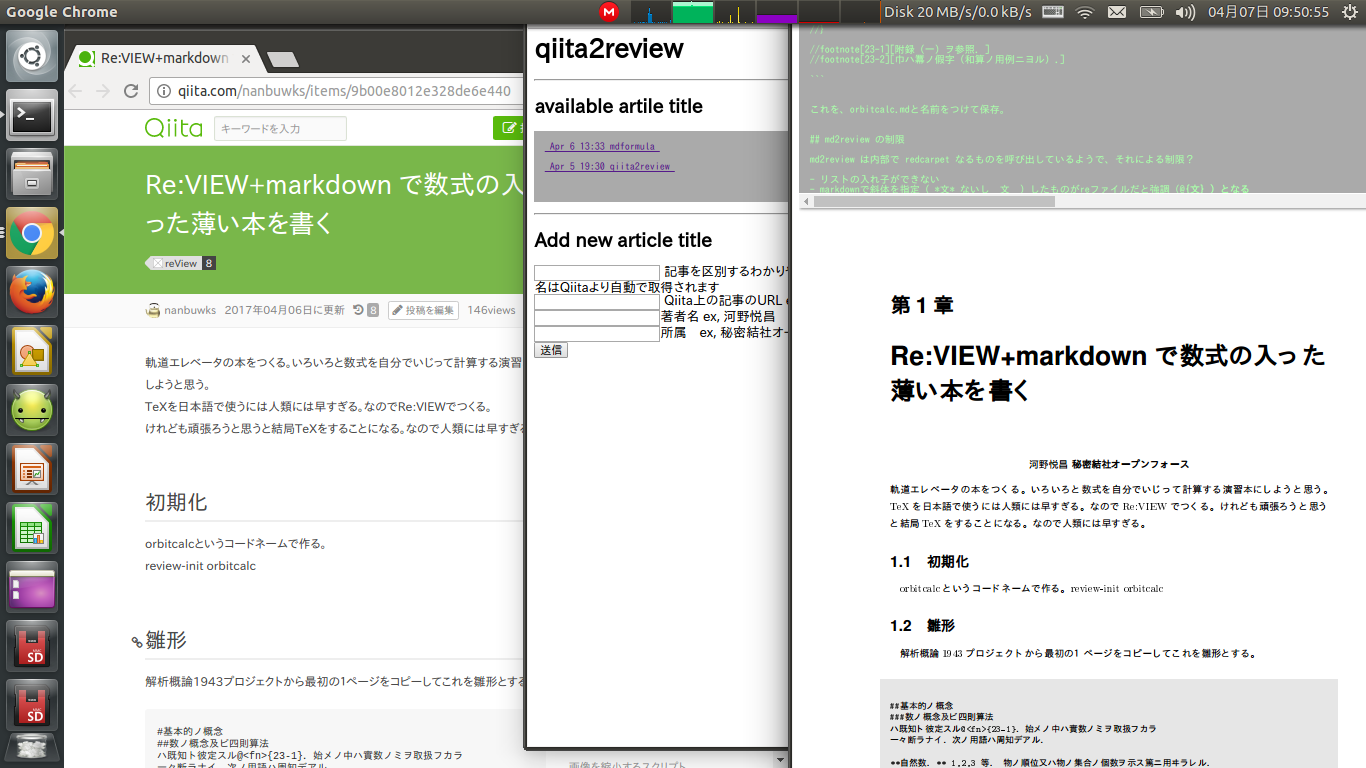
\includegraphics[width=\maxwidth]{./images/80cbc196-d4ef-b880-733c-54d0a8aa45bb.png}
\caption{Screenshot from 2017{-}04{-}07 09{-}50{-}56.png}
\label{image:howtoQiita2Review:80cbc196-d4ef-b880-733c-54d0a8aa45bb}
\end{reviewimage}

\section{qiita2review とは}
\label{sec:1-1}

\begin{itemize}
\item Qiita で記事を執筆してもらってRe:VIEWでPDFにするオンラインシステム。
\item グループ作業で技術情報をマルチ展開するために。
\item Qiita だと学習コスト少、画像楽だし数式も使える。
\item PDF作ると同時にちゃんとしたWebコンテンツを公開できる。
\end{itemize}

\section{管理者がはじめにやること}
\label{sec:1-2}

サーバにインストール、認証設定、サーバアドレスの執筆者への周知。

\section{執筆者がやること}
\label{sec:1-3}

\subsection*{Qiitaに記事を書く}
\addcontentsline{toc}{subsection}{Qiitaに記事を書く}
\label{sec:1-3-1}

後々PDFにするために、ちょっと気をつける点。

\subsubsection*{画像}
\label{sec:1-3-1-1}

画像はそのままだと100\%になり、紙媒体では大きすぎることが多い。縮小設定をしておく。
通常の画像は

\begin{reviewemlist}
![ファイル名](images/......8d78.jpeg)
\end{reviewemlist}

のようになってますが

\begin{reviewemlist}
[]( scale=0.5 )![ファイル名](https://qiita{-}image{-}store.s3.amazonaws.com/0/......8d78.jpeg)

\end{reviewemlist}

のように頭に\texttt{scale=0.5 )}をつけると、Qiitaでは100\%,PDFにしたときには50\%サイズになります。

\subsubsection*{Re:VIEWの制限}
\label{sec:1-3-1-2}

PDF化に使用しているRe:VIEW受け付けない書式にならないように注意
{-} コメントの入れ子
{-} コードブロック開始前に改行を入れる

コードブロック開始前に改行がない場合、Markdownとしてもヘンになることが多いので改行を入れる習慣をつけよう。

\subsection*{Qiitaに記事が書けたら}
\addcontentsline{toc}{subsection}{Qiitaに記事が書けたら}
\label{sec:1-3-2}

PDF化の確認をします。

qiita2reviewサーバページから、記事一覧が見えます。

画面下部の
「Add new article title」
のフォームに入力して送信すると新しい記事が登録できる。

(認証が必要)

Qiitaの1記事ごとにPDFになる。別刷りのようなイメージ。

\section{原稿が集まったら}
\label{sec:1-4}

本としての装丁は管理者が行います。
1記事になっているものはそれぞれ章にして、まとめて1冊としてレンダリング→印刷
管理者のお仕事となります。今のところはサーバにsshログインしてRe:VIEWを使って手作業です。

\chapter{Qiitaで数式を書きましょう}
\label{chap:QiitaFormula}
 \begin{center} 
河野悦昌  \textbf{オープンフォース}

 \end{center} 
\section{TeX式を簡単に作成する}
\label{sec:2-1}

https://webdemo.myscript.com/views/math.html\#
ここで数式を手書きで書くとTeX式に直してくれます

\begin{reviewimage}
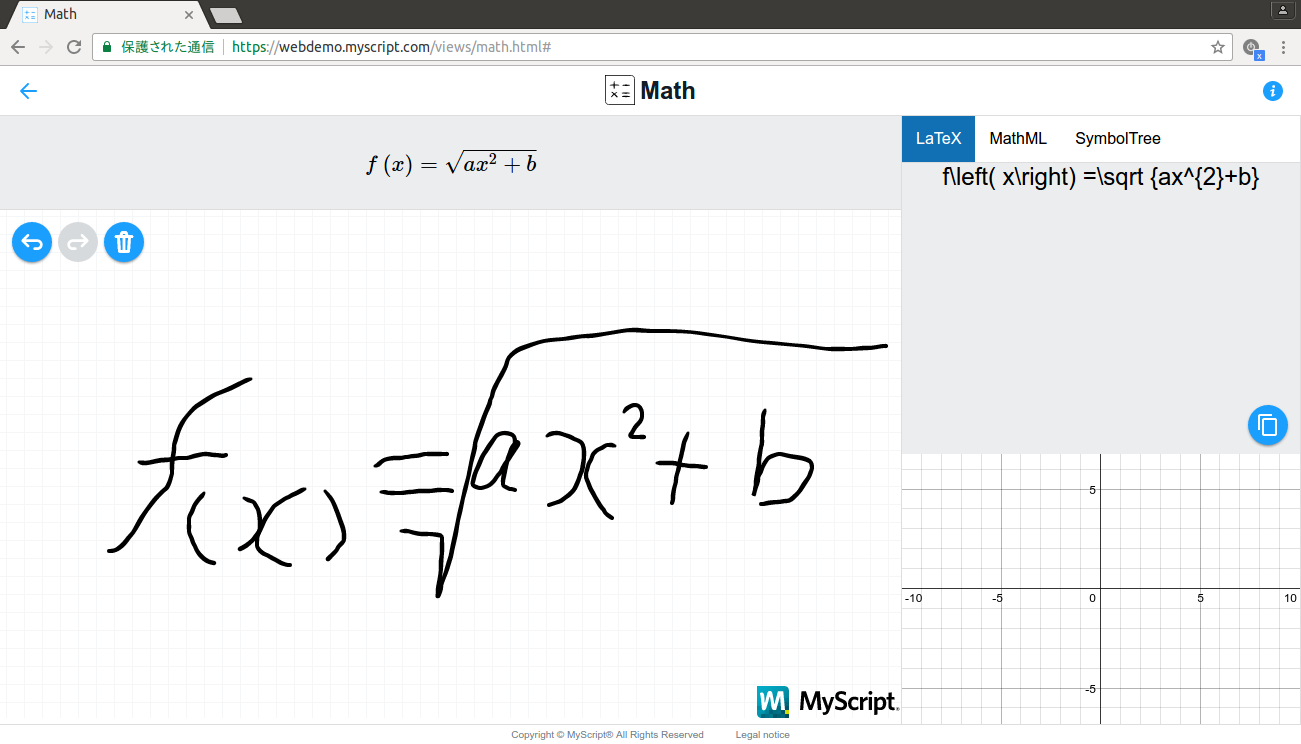
\includegraphics[width=\maxwidth]{./images/f7182c75-f4fe-07a4-6d54-c76f5d514db8.png}
\caption{image}
\label{image:QiitaFormula:f7182c75-f4fe-07a4-6d54-c76f5d514db8}
\end{reviewimage}

\subsection*{Qiitaで書く}
\addcontentsline{toc}{subsection}{Qiitaで書く}
\label{sec:2-1-1}

先のページで作ったLaTeX式をコピーします。

\begin{reviewemlist}
f\reviewbackslash{}left( x\reviewbackslash{}right) =\reviewbackslash{}sqrt \{ax\textasciicircum{}\{2\}+b\}


\end{reviewemlist}

この数式をQiitaで書いてみます。

\begin{quote}
「 TeXで作った式 \textdollar{} f\reviewbackslash{}left( x\reviewbackslash{}right) =\reviewbackslash{}sqrt \{ax\textasciicircum{}\{2\}+b\} \textdollar{} です 」

\end{quote}

と書くと

「 TeXで作った式  $ f\left( x\right) =\sqrt {ax^{2}+b} $  です 」

となります。

ブロック書式で書くには

\begin{quote}
```math

「 TeXで作った式  f\reviewbackslash{}left( x\reviewbackslash{}right) =\reviewbackslash{}sqrt \{ax\textasciicircum{}\{2\}+b\}  です 」

```

\end{quote}

と書くと

\begin{equation*}
「 TeXで作った式  f\left( x\right) =\sqrt {ax^{2}+b}  です 」
\end{equation*}

となります。

\chapter{AWS上にRe:VIEW環境を構築する}
\label{chap:AWSReVIEW}

AWS 上に Re:VIEW 環境を構築してみました。

\section{環境}
\label{sec:3-1}

\begin{itemize}
\item T2.micro
\item Ubuntu 16.04 64bit(Ubuntu 14.04から dist{-}upgreadeをかけています。)既に ruby や rack は別の用事でインストール終えていました。
\end{itemize}

\section{インストール}
\label{sec:3-2}

\begin{reviewemlist}
gem install review
gem install md2review
\end{reviewemlist}

試してみます

\begin{reviewemlist}
review{-}init testwrite
cd testwrite
rake pdf
\end{reviewemlist}

エラー

\begin{reviewemlist}
review{-}pdfmaker config.yml
compiling testwrite.tex
/var/lib/gems/2.3.0/gems/review{-}2.2.0/lib/review/pdfmaker.rb:42:in `system\textunderscore{}or\textunderscore{}raise': failed to run command: ebb cover.jpg (RuntimeError)
    from /var/lib/gems/2.3.0/gems/review{-}2.2.0/lib/review/pdfmaker.rb:276:in `block in copy\textunderscore{}images'
    from /var/lib/gems/2.3.0/gems/review{-}2.2.0/lib/review/pdfmaker.rb:269:in `chdir'
    from /var/lib/gems/2.3.0/gems/review{-}2.2.0/lib/review/pdfmaker.rb:269:in `copy\textunderscore{}images'
    from /var/lib/gems/2.3.0/gems/review{-}2.2.0/lib/review/pdfmaker.rb:235:in `generate\textunderscore{}pdf'
    from /var/lib/gems/2.3.0/gems/review{-}2.2.0/lib/review/pdfmaker.rb:132:in `execute'
    from /var/lib/gems/2.3.0/gems/review{-}2.2.0/lib/review/pdfmaker.rb:86:in `execute'
    from /var/lib/gems/2.3.0/gems/review{-}2.2.0/bin/review{-}pdfmaker:18:in `\textless{}top (required)\textgreater{}'
    from /usr/local/bin/review{-}pdfmaker:22:in `load'
    from /usr/local/bin/review{-}pdfmaker:22:in `\textless{}main\textgreater{}'
rake aborted!
Command failed with status (1): [review{-}pdfmaker config.yml...]
/home/ubuntu/testwrite/Rakefile:60:in `block in \textless{}top (required)\textgreater{}'
/var/lib/gems/1.9.1/gems/rake{-}11.2.2/exe/rake:27:in `\textless{}top (required)\textgreater{}'
Tasks: TOP =\textgreater{} pdf =\textgreater{} book.pdf
(See full trace by running task with {-}{-}trace)
\end{reviewemlist}

Re:VIEWは2.0からはuplatexを使うらしいので、インストールします。

\begin{reviewemlist}
\textdollar{} apt{-}cache search uplatex
texlive{-}lang{-}cjk {-} TeX Live: Chinese/Japanese/Korean
\end{reviewemlist}

ということなので、

\begin{reviewemlist}
\textdollar{} sudo apt{-}get install texlive{-}lang{-}cjk
sudo: unable to resolve host ip{-}172{-}30{-}0{-}222
Reading package lists... Done
Building dependency tree
Reading state information... Done
The following extra packages will be installed:
  fontconfig{-}config fonts{-}dejavu{-}core fonts{-}ipaexfont{-}gothic
  fonts{-}ipaexfont{-}mincho fonts{-}ipafont{-}gothic fonts{-}ipafont{-}mincho
  fonts{-}lmodern ghostscript gsfonts ko.tex{-}extra{-}hlfont latex{-}beamer
  latex{-}cjk{-}all latex{-}cjk{-}chinese latex{-}cjk{-}chinese{-}arphic{-}bkai00mp
  latex{-}cjk{-}chinese{-}arphic{-}bsmi00lp latex{-}cjk{-}chinese{-}arphic{-}gbsn00lp
  latex{-}cjk{-}chinese{-}arphic{-}gkai00mp latex{-}cjk{-}common latex{-}cjk{-}japanese
  latex{-}cjk{-}japanese{-}wadalab latex{-}cjk{-}korean latex{-}cjk{-}thai latex{-}xcolor
  libavahi{-}client3 libavahi{-}common{-}data libavahi{-}common3 libcairo2 libcups2
  libcupsfilters1 libcupsimage2 libdatrie1 libdrm{-}intel1 libdrm{-}nouveau2
  libdrm{-}radeon1 libfile{-}basedir{-}perl libfile{-}desktopentry{-}perl
  libfile{-}mimeinfo{-}perl libfontconfig1 libfontenc1 libgl1{-}mesa{-}dri
  libgl1{-}mesa{-}glx libglapi{-}mesa libgraphite2{-}3 libgs9 libgs9{-}common
  libharfbuzz0b libice6 libijs{-}0.35 libjbig0 libjbig2dec0 libjpeg{-}turbo8
  libjpeg8 libkpathsea6 liblcms2{-}2 libllvm3.4 libpaper{-}utils libpaper1
  libpciaccess0 libpixman{-}1{-}0 libpoppler44 libptexenc1 libsm6 libtcl8.6
  libtiff5 libtk8.6 libtxc{-}dxtn{-}s2tc0 libutempter0 libx11{-}xcb1 libxaw7
  libxcb{-}dri2{-}0 libxcb{-}dri3{-}0 libxcb{-}glx0 libxcb{-}present0 libxcb{-}render0
  libxcb{-}shape0 libxcb{-}shm0 libxcb{-}sync1 libxcomposite1 libxcursor1
  libxdamage1 libxfixes3 libxft2 libxi6 libxinerama1 libxmu6 libxpm4
  libxrandr2 libxrender1 libxshmfence1 libxss1 libxt6 libxtst6 libxv1
  libxxf86dga1 libxxf86vm1 lmodern luatex pgf poppler{-}data preview{-}latex{-}style
  prosper ps2eps ruby swath tcl tcl8.6 tex{-}common texlive{-}base
  texlive{-}binaries texlive{-}extra{-}utils texlive{-}font{-}utils
  texlive{-}generic{-}recommended texlive{-}lang{-}other texlive{-}latex{-}base
  texlive{-}latex{-}base{-}doc texlive{-}latex{-}extra texlive{-}latex{-}extra{-}doc
  texlive{-}latex{-}recommended texlive{-}latex{-}recommended{-}doc texlive{-}luatex
  texlive{-}pictures texlive{-}pictures{-}doc texlive{-}pstricks texlive{-}pstricks{-}doc
  tk tk8.6 x11{-}common x11{-}utils x11{-}xserver{-}utils xbitmaps xdg{-}utils xterm
Suggested packages:
  ghostscript{-}x hpijs hbf{-}cns40{-}b5 hbf{-}jfs56 fonts{-}arphic{-}bkai00mp
  fonts{-}arphic{-}bsmi00lp fonts{-}arphic{-}gbsn00lp fonts{-}arphic{-}gkai00mp
  hbf{-}kanji48 cups{-}common libglide3 fonts{-}droid liblcms2{-}utils poppler{-}utils
  fonts{-}arphic{-}ukai fonts{-}arphic{-}uming fonts{-}unfonts{-}core pdf{-}viewer
  postscript{-}viewer ri ruby{-}dev libthai{-}data tcl{-}tclreadline debhelper perl{-}tk
  chktex fragmaster xindy latexdiff lacheck latexmk dvidvi purifyeps dvipng
  t1utils psutils latex{-}fonts{-}sipa{-}arundina libfile{-}which{-}perl python{-}pygments
  dot2tex libtcltk{-}ruby mesa{-}utils nickle cairo{-}5c xorg{-}docs{-}core gvfs{-}bin
  xfonts{-}cyrillic
Recommended packages:
  wish
The following NEW packages will be installed:
  fontconfig{-}config fonts{-}dejavu{-}core fonts{-}ipaexfont{-}gothic
  fonts{-}ipaexfont{-}mincho fonts{-}ipafont{-}gothic fonts{-}ipafont{-}mincho
  fonts{-}lmodern ghostscript gsfonts ko.tex{-}extra{-}hlfont latex{-}beamer
  latex{-}cjk{-}all latex{-}cjk{-}chinese latex{-}cjk{-}chinese{-}arphic{-}bkai00mp
  latex{-}cjk{-}chinese{-}arphic{-}bsmi00lp latex{-}cjk{-}chinese{-}arphic{-}gbsn00lp
  latex{-}cjk{-}chinese{-}arphic{-}gkai00mp latex{-}cjk{-}common latex{-}cjk{-}japanese
  latex{-}cjk{-}japanese{-}wadalab latex{-}cjk{-}korean latex{-}cjk{-}thai latex{-}xcolor
  libavahi{-}client3 libavahi{-}common{-}data libavahi{-}common3 libcairo2 libcups2
  libcupsfilters1 libcupsimage2 libdatrie1 libdrm{-}intel1 libdrm{-}nouveau2
  libdrm{-}radeon1 libfile{-}basedir{-}perl libfile{-}desktopentry{-}perl
  libfile{-}mimeinfo{-}perl libfontconfig1 libfontenc1 libgl1{-}mesa{-}dri
  libgl1{-}mesa{-}glx libglapi{-}mesa libgraphite2{-}3 libgs9 libgs9{-}common
  libharfbuzz0b libice6 libijs{-}0.35 libjbig0 libjbig2dec0 libjpeg{-}turbo8
  libjpeg8 libkpathsea6 liblcms2{-}2 libllvm3.4 libpaper{-}utils libpaper1
  libpciaccess0 libpixman{-}1{-}0 libpoppler44 libptexenc1 libsm6 libtcl8.6
  libtiff5 libtk8.6 libtxc{-}dxtn{-}s2tc0 libutempter0 libx11{-}xcb1 libxaw7
  libxcb{-}dri2{-}0 libxcb{-}dri3{-}0 libxcb{-}glx0 libxcb{-}present0 libxcb{-}render0
  libxcb{-}shape0 libxcb{-}shm0 libxcb{-}sync1 libxcomposite1 libxcursor1
  libxdamage1 libxfixes3 libxft2 libxi6 libxinerama1 libxmu6 libxpm4
  libxrandr2 libxrender1 libxshmfence1 libxss1 libxt6 libxtst6 libxv1
  libxxf86dga1 libxxf86vm1 lmodern luatex pgf poppler{-}data preview{-}latex{-}style
  prosper ps2eps ruby swath tcl tcl8.6 tex{-}common texlive{-}base
  texlive{-}binaries texlive{-}extra{-}utils texlive{-}font{-}utils
  texlive{-}generic{-}recommended texlive{-}lang{-}cjk texlive{-}lang{-}other
  texlive{-}latex{-}base texlive{-}latex{-}base{-}doc texlive{-}latex{-}extra
  texlive{-}latex{-}extra{-}doc texlive{-}latex{-}recommended
  texlive{-}latex{-}recommended{-}doc texlive{-}luatex texlive{-}pictures
  texlive{-}pictures{-}doc texlive{-}pstricks texlive{-}pstricks{-}doc tk tk8.6
  x11{-}common x11{-}utils x11{-}xserver{-}utils xbitmaps xdg{-}utils xterm
0 upgraded, 133 newly installed, 0 to remove and 0 not upgraded.
Need to get 852 MB of archives.
After this operation, 1,625 MB of additional disk space will be used.
Do you want to continue? [Y/n] y
\end{reviewemlist}

さて、どうかな?

\begin{reviewemlist}
\textdollar{} rake pdf
・
・
・
\textless{}to be read again\textgreater{}
                   relax
l.100 \reviewbackslash{}fontencoding\reviewbackslash{}encodingdefault\reviewbackslash{}selectfont

?
\end{reviewemlist}

と出たので、フォントをインストール

\begin{reviewemlist}
\textdollar{} sudo apt{-}get install texlive{-}fonts{-}recommended
\end{reviewemlist}

として、
@\textless{}tt\textgreater{}\{
rake pdf
\}
とすると、

book.pdfができました。

\chapter{Re:VIEW+markdown で数式の入った薄い本を書く}
\label{chap:mdformula}
 \begin{center} 
河野悦昌  \textbf{秘密結社オープンフォース}

 \end{center} 
軌道エレベータの本をつくる。いろいろと数式を自分でいじって計算する演習本にしようと思う。
TeXを日本語で使うには人類には早すぎる。なのでRe:VIEWでつくる。
けれども頑張ろうと思うと結局TeXをすることになる。なので人類には早すぎる。

\section{初期化}
\label{sec:4-1}

orbitcalcというコードネームで作る。
review{-}init orbitcalc

\section{雛形}
\label{sec:4-2}

解析概論1943プロジェクトから最初の1ページをコピーしてこれを雛形とする。

\begin{reviewemlist}

\#\#基本的ノ概念
\#\#\#数ノ概念及ビ四則算法
ハ既知ト彼定スル@\textless{}fn\textgreater{}\{23{-}1\}.始メノ中ハ實数ノミヲ取扱フカラ
一々断ラナイ.次ノ用語ハ周知デアル.

**自然数.** 1,2,3 等. 物ノ順位又ハ物ノ集合ノ個数ヲ示ス篤ニ用ヰラレル.

**整数.** 0,±1,±2等. 自然数ハ正ノ整数デアル.

**有理数.**0及ビ @\textless{}m\textgreater{}\{\reviewbackslash{}pm \reviewbackslash{}dfrac \{a\reviewbackslash{}\reviewbackslash{}\} \{b\reviewbackslash{}\reviewbackslash{}\}\}子,但α,b ハ自然数. b=1ナルトキ,ソレハ整数デアル.

**無理数.**有理数以外ノ責数.例ヘバ

//texequation\{
\reviewbackslash{}begin\{array\}\{l\}
\reviewbackslash{}sqrt \{2\}=1.4142135\reviewbackslash{}ldots,\reviewbackslash{}\reviewbackslash{}\reviewbackslash{}
e=2.718281828…,\reviewbackslash{}\reviewbackslash{}\reviewbackslash{}
pi=3.1415926535…
\reviewbackslash{}end\{array\}
//\}



(但,ソレラガ有理数デナイコトハ護明ヲ要スル)
  十進法.賓数ヲ十進法デ表ハスコトモ周知デアル.有理数ヲ十進法デ表ハセバ,数字
ハ有限カ,又ハ無限ナラバ循環小数ニナル.但,有限位数ノ十進数ヲ循環小数ノ形二表ハス
コトモ出来ル.例ヘバ0.6= 0.5999….無理数ヲ十進法デ表ハスナラバ,無限ノ位数ヲ要
シ,数字ハ決シテ循環シナイ.
  吾々ガ十進法ニヨツテ数ヲ表ハズニ至ツタノハ,手指ノ数ニソノ原因ガアルノデアラ
ウガ,理論上ハ1以外ノ任意ノ自然数ヲ基本トシテ,十進法ト同様ノ方法ニヨツテ,数ヲ表
ハスコトガ出来ル.
  特ニ二進法デハ,数字ハ0ト1トダケデ足ル.有理数ヲ二進法デ表ハセバ,分母ガ2
ノ巾@\textless{}fn\textgreater{}\{23{-}2\}ニナルモノノ外ハ,循環二進数ニナル.
//texequation\{
\reviewbackslash{}left[ 例\reviewbackslash{}right] \reviewbackslash{}dfrac \{5\} \{8\}=\reviewbackslash{}dfrac \{1\} \{2\}+\reviewbackslash{}dfrac \{1\} \{2\textasciicircum{}\{3\}\}=\reviewbackslash{}left( \reviewbackslash{}begin\{matrix\} 0.101\reviewbackslash{}end\{matrix\} \reviewbackslash{}right)
//\}

//footnote[23{-}1][附録(一)ヲ参照.]
//footnote[23{-}2][巾ハ羃ノ假字(和算ノ用例ニヨル).]

\end{reviewemlist}

これを、orbitcalc.mdと名前をつけて保存。

\section{md2review の制限}
\label{sec:4-3}

md2review は内部で redcarpet なるものを呼び出しているようで、それによる制限?

\begin{itemize}
\item リストの入れ子ができない
\item markdownで斜体を指定 ( \textbf{文} ないし \textbf{文} ) したものがreファイルだと強調 (\textbf{文} ) となる
\end{itemize}

このほか、reファイルでは引用ブロック( //quote\{ 文 \} )の入れ子をするとエラーになるので、二重引用しているmarkdownをmd2reviewして作ったreファイルはエラーが出る。

\section{TeXの機能を使って中央揃えを実現する}
\label{sec:4-4}

\begin{reviewemlist}
//raw[\textbar{}latex\textbar{} \reviewbackslash{}begin\{center\} 中央揃えにしたい文 \reviewbackslash{}end\{center\} ]
\end{reviewemlist}

\begin{reviewemlist}
//raw[\textbar{}latex\textbar{} \reviewbackslash{}begin\{center\} ]
**筆頭著者** 共著者 *所属*
//raw[\textbar{}latex\textbar{} \reviewbackslash{}end\{center\} ]
\end{reviewemlist}

のようにすればいい。しかしながら
\texttt{//raw} の部分がmarkdownビューの時にゴミとして出てくる。なのでここらへんはTeXコンパイル時にフィルターとして活用するなど。

qiitaの場合は以下のようにすると中央揃えとなる。

\begin{equation*}
中央揃え
\end{equation*}

このようなフォーマットを通すためのフィルタは以下の通り

\begin{reviewemlist}
\textgreater{} ```math
\textgreater{} \reviewbackslash{}left[ 例\reviewbackslash{}right] \reviewbackslash{}dfrac \{5\} \{8\}=\reviewbackslash{}dfrac \{1\} \{2\}+\reviewbackslash{}dfrac \{1\}   \{2\textasciicircum{}\{3\}\}=\reviewbackslash{}left( \reviewbackslash{}begin\{matrix\} 0.101\reviewbackslash{}end\{matrix\} \reviewbackslash{}right)
\textgreater{} ```
\end{reviewemlist}

↓

\begin{reviewemlist}
//texequation\{
\reviewbackslash{}left[ 例\reviewbackslash{}right] \reviewbackslash{}dfrac \{5\} \{8\}=\reviewbackslash{}dfrac \{1\} \{2\}+\reviewbackslash{}dfrac \{1\} \{2\textasciicircum{}\{3\}\}=\reviewbackslash{}left( \reviewbackslash{}begin\{matrix\} 0.101\reviewbackslash{}end\{matrix\} \reviewbackslash{}right)
//\}
\end{reviewemlist}

インライン命令`a{-}\textdollar{}\textdollar{}

\begin{reviewemlist}
\textdollar{}\reviewbackslash{}pm \reviewbackslash{}dfrac \{a\} \{b\}\textdollar{}
\end{reviewemlist}

↓

\begin{reviewemlist}
@\textless{}m\textgreater{}\{\reviewbackslash{}pm \reviewbackslash{}dfrac \{a\reviewbackslash{}\reviewbackslash{}\} \{b\reviewbackslash{}\reviewbackslash{}\}\}
\end{reviewemlist}

 

\section{画像を縮小するスクリプト}
\label{sec:4-5}

写真や図も入れる。写真や図を、markdownの段階でプレビューしやすい形で作りたい。
通常の書き方

\begin{reviewemlist}
![test](images/test.png  "" )
\end{reviewemlist}

だけど、このままだと縮小できない。なのでスクリプトで何とかする。
@\textless{}tt\textgreater{}\{
通常の書き方
![テスト](images/test.png  "" )
拡張した書き方
[scale=0.5]![テスト](./images/test.png  "" )
\}
↓md2reviewを通す

\begin{reviewemlist}
通常の書き方
//image[test][テスト]\{
//\}
拡張した書き方
//[test][テスト][scale=0.5]\{
//\}
\end{reviewemlist}

となる。
これを、
↓

\begin{reviewemlist}
通常の書き方
//image[test][テスト]\{
//\}
拡張した書き方
//image[test][テスト][scale=0.5]\{
//\}
\end{reviewemlist}

とするスクリプト。

\begin{reviewemlist}
\#\#!/usr/bin/env ruby
while line = gets
  line.chomp!
  if md1 = line.match(/\textasciicircum{}\reviewbackslash{}[.*?\reviewbackslash{}]/)
    if md2 = line.match(/\reviewbackslash{}/\reviewbackslash{}/(.+)\reviewbackslash{}]/)
      print md2[0],md1[0],"\{\reviewbackslash{}n"
    else
      puts line
    end
  else
    puts line
  end
end

\end{reviewemlist}

scalemd.rb

\begin{reviewemlist}
\#\#!/usr/bin/env ruby
while line = gets
  line.chomp!
  if md1 = line.match(/\textasciicircum{}\reviewbackslash{}[.*?\reviewbackslash{}]/)
    if md2 = line.match(/\reviewbackslash{}/\reviewbackslash{}/(.+)\reviewbackslash{}]/)
      print md2[0],md1[0],"\{\reviewbackslash{}n"
    else
      puts line
    end
  else
    puts line
  end
end

\end{reviewemlist}

使い方
@\textless{}tt\textgreater{}\{
md2review orbitcalc.md \textbar{} ruby scalemd.rb \textgreater{} orbitcalc.re
\}

\section{config.ymlやcover.jpgを入れ替える}
\label{sec:4-6}

cover.jpg は1110x1,840 は2ページ目に配置された。1101x1825だとOK。

\section{ひたすら書く}
\label{sec:4-7}

(明日から頑張る)

\section{Tips}
\label{sec:4-8}

\subsection*{数式を書く}
\addcontentsline{toc}{subsection}{数式を書く}
\label{sec:4-8-1}

Web Equation
を使って、手書き数式をTEXに変換してくれる。
https://webdemo.myscript.com/\#/demo/equation
紹介ページ
http://gigazine.net/news/20120203{-}latex{-}mathml{-}web{-}equation/

ここで書いた数式をゲット

\begin{reviewemlist}

g=r\reviewbackslash{}omega \textasciicircum{}\{2\}

\end{reviewemlist}

ブロック要素として数式を入れるには

\begin{reviewemlist}
//texequation\{
g=r\reviewbackslash{}omega \textasciicircum{}\{2\}
//\}
\end{reviewemlist}

というように囲めばいい

インライン要素として数式を入れるには

\begin{reviewemlist}
@\textless{}m\textgreater{}\{g=r\reviewbackslash{}omega \textasciicircum{}\{2\reviewbackslash{}\reviewbackslash{}\}\}
\end{reviewemlist}

というように、閉じ大括弧の前にエスケープを2つ入れる。人類にはまだ早い。

\subsection*{コードブロック中に \texttt{//\}} が書けない}
\addcontentsline{toc}{subsection}{コードブロック中に \texttt{//\}} が書けない}
\label{sec:4-8-2}

markdown 上のコードブロック中には \texttt{//\}} は問題なくかけるのだけれど、Re:VIEW形式に変換するとコードブロックがそこで閉じてしまい、エラーとなる。Re:VIEW のブロック構文は\texttt{//\}} を閉じタグになっているのでRe:VIEWの構文を解説する文書が Re:VIEWで書けないということになってしまう。

これは Re:VIEW形式の仕様の問題かな。

\begin{quote}
//embedブロック命令はブロック内の文字列をそのまま文書中に埋め込みます。エスケープされる文字はありません。

\end{quote}

「Re:VIEW フォーマットガイド」
https://github.com/kmuto/review/blob/master/doc/format.ja.md

コードブロック中の書き方でどうにかできないかと思ったけれどもエスケープできないのでこれはどうしようもない。仕方がないので、markdownの段階でフィルタを通すことにした。コードブロック中に \texttt{//\}} が存在するようなら各行頭にスペースを入れるようにした。

slash2braceincode.rb

\begin{reviewemlist}
@\textless{}raw\textgreater{}\{@\}\textless{}fn\textgreater{}\{23{-}1\}
//@\textless{}raw\textgreater{}\{\}\}
\end{reviewemlist}

↓

\begin{reviewemlist}
@\textless{}fn\textgreater{}\{23{-}1\}
//\}
\end{reviewemlist}

実は下の//\}は何も出力していない。パーサを邪魔しているだけ。

あたまの
@\textless{}tt\textgreater{}\{
\}
```
の前に改行が無いとRe:VIEWでは

\begin{reviewemlist}
//emlist\{
\end{reviewemlist}

ではなく

\begin{reviewemlist}
@\textless{}tt\textgreater{}\{
\end{reviewemlist}

となる。ここにインライン命令が入るとmd2reviewが余計なエスケープをつけてコンパイルできなくなる。

なので改行をつけよう。

また、Re:VIEWの命令に誤解釈されるものを本文に書くとおかしくなる。

\subsection*{markdown と Re:VIEWファイルの違い}
\addcontentsline{toc}{subsection}{markdown と Re:VIEWファイルの違い}
\label{sec:4-8-3}

\subsubsection*{エンターの扱い}
\label{sec:4-8-3-1}

markdown → 改行となる
Re:VIEW → 空白となる

\chapter{組版システムReVIEWでQiitaから同人誌原稿を作る}
\label{chap:qiita2review}
 \begin{center} 
河野悦昌  \textbf{秘密結社オープンフォース 送信}

 \end{center} 
\section{markdownからReVIEW}
\label{sec:5-1}

ReVIEW+markdown で数式の入った薄い本を書く
http://qiita.com/nanbuwks/items/9b00e8012e328de6e440
というのを書きました。

何人かでこういうのやるときに、オンライン投稿するやりかたを考えます。

\section{Qiitaで書くメリット}
\label{sec:5-2}

Qiita ってよくできていて、割とラフな操作でもいい感じに作ってくれます。

\begin{itemize}
\item オンラインで投稿、書いてる途中でリアルタイムにレンダリング結果を確認
\item 画像ドラッグ\&ドロップで投稿できる
\item URLとか自動でリンクに変換してくれる
\end{itemize}

これを使うやり方を考えてみました。

\section{catalog.yml}
\label{sec:5-3}

章立てはこうなってます

\begin{reviewemlist}
PREDEF:

CHAPS:
  {-} 1.re

APPENDIX:

POSTDEF:
\end{reviewemlist}

ここの、CHAPSに複数人の原稿を登録するという感じです。

\section{ひとつの記事を元に原稿を作ってみる}
\label{sec:5-4}

Pi board (Single Board Computer) and Allwinner
http://qiita.com/nanbuwks/items/7f5fd126b8581e6d1a74

を元にしてみます。

まず、

\begin{reviewemlist}
review{-}init piallwinner
cd piallwinner
\end{reviewemlist}

catalog.ymlと config.yml を編集しておきます。

図をダウンロードします

\begin{reviewemlist}
cd images
wget http://qiita.com/nanbuwks/items/7f5fd126b8581e6d1a74 {-}k {-}H {-}r {-}l 1 {-}nH {-}nd {-}A png,PNG,jpg,JPG,jpeg,JPEG,html  {-}R txt
cd ..
\end{reviewemlist}

markdownファイルをダウンロードします。

\begin{reviewemlist}
wget http://qiita.com/nanbuwks/items/7f5fd126b8581e6d1a74.md
\end{reviewemlist}

imgファイルをローカルに変換します。

\begin{reviewemlist}
ruby qiitamd.rb 7f5fd126b8581e6d1a74.md \textgreater{} 1.md
md2review 1.md \textgreater{} 1.re
rake pdf
\end{reviewemlist}

変換するスクリプト qiitamd.rb です

\begin{reviewemlist}
\#\#!/usr/bin/env ruby

while line = gets
  line.chomp!
  if md1 = line.match(/(\textasciicircum{}!\reviewbackslash{}[.*?\reviewbackslash{}]\reviewbackslash{}()/)
    if md2 = line.match(/([\textasciicircum{}\reviewbackslash{}/]*\reviewbackslash{}))/)
\#\#      puts line
\#\#      print md1[0],"\reviewbackslash{}n"
\#\#      print md1[1],"\reviewbackslash{}n"
\#\#      print md2[0],"\reviewbackslash{}n"
\#\#      print md2[1],"\reviewbackslash{}n"
\#\#      print "\reviewbackslash{}n"
\#\#      print md2[0],md1[0],"\{\reviewbackslash{}n"
      print md1[0]
      print "images/"
      print md2[1]
      print "\reviewbackslash{}n"
    else
      puts line
    end
  else
   puts line
  end
end

\end{reviewemlist}

\section{複数の記事を元に原稿を作ってみる}
\label{sec:5-5}

\begin{reviewemlist}
PREDEF:

CHAPS:
  {-} 1.re
  {-} 2.re
  {-} 3.re

APPENDIX:

POSTDEF:
\end{reviewemlist}

として、2.re や 3.re に上のような原稿を当てはめるといいでしょう。

\section{画像を縮小する}
\label{sec:5-6}

Qiitaは画像をアップロードすると、はみ出る画像は横幅100\%でビューするように画面を作ってくれます。紙媒体の場合は多くは100\%だと良くないですね。50\%ぐらいの大きさを使うようにするには?

通常の画像をアップロードすると以下のようなmarkdownとなります。
@\textless{}tt\textgreater{}\{
![ファイル名](images/c19f0873{-}8b39{-}9405{-}1486{-}8cfd43e38d78.jpeg)
\}

\begin{reviewimage}
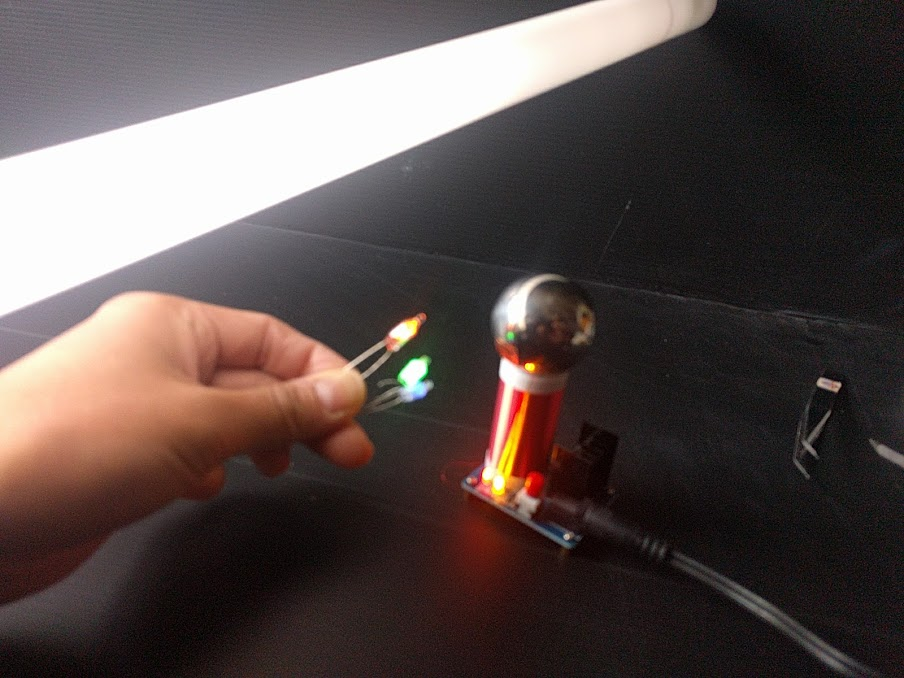
\includegraphics[width=\maxwidth]{./images/c19f0873-8b39-9405-1486-8cfd43e38d78.jpeg}
\caption{ファイル名}
\label{image:qiita2review:c19f0873-8b39-9405-1486-8cfd43e38d78}
\end{reviewimage}

Qiitaでは、imgタグに書き換えると小さくなります。
@\textless{}tt\textgreater{}\{
\textless{}img width="50\%" alt="ファイル名" src="https://qiita{-}image{-}store.s3.amazonaws.com/0/139524/c19f0873{-}8b39{-}9405{-}1486{-}8cfd43e38d78.jpeg"\textgreater{}
\}

\textless{}img width="50\%" alt="ファイル名" src="https://qiita{-}image{-}store.s3.amazonaws.com/0/139524/c19f0873{-}8b39{-}9405{-}1486{-}8cfd43e38d78.jpeg"\textgreater{}

この解決方法は、GitHubなどでも同様です。
タグをいちいち書き換えないといけないのでメンドクサイですね。
markdownの拡張でできないかと思ったのですがそういうのは無さそうです。

仕方がないので、Qiita上では100\%で表示されるけれども、PDFに変換した時に任意の大きさになるようにする。

「画像を初期化するスクリプト」
http://qiita.com/nanbuwks/items/9b00e8012e328de6e440\#\%E7\%94\%BB\%E5\%83\%8F\%E3\%82\%92\%E7\%B8\%AE\%E5\%B0\%8F\%E3\%81\%99\%E3\%82\%8B\%E3\%82\%B9\%E3\%82\%AF\%E3\%83\%AA\%E3\%83\%97\%E3\%83\%88

を使うと、

\begin{reviewimage}
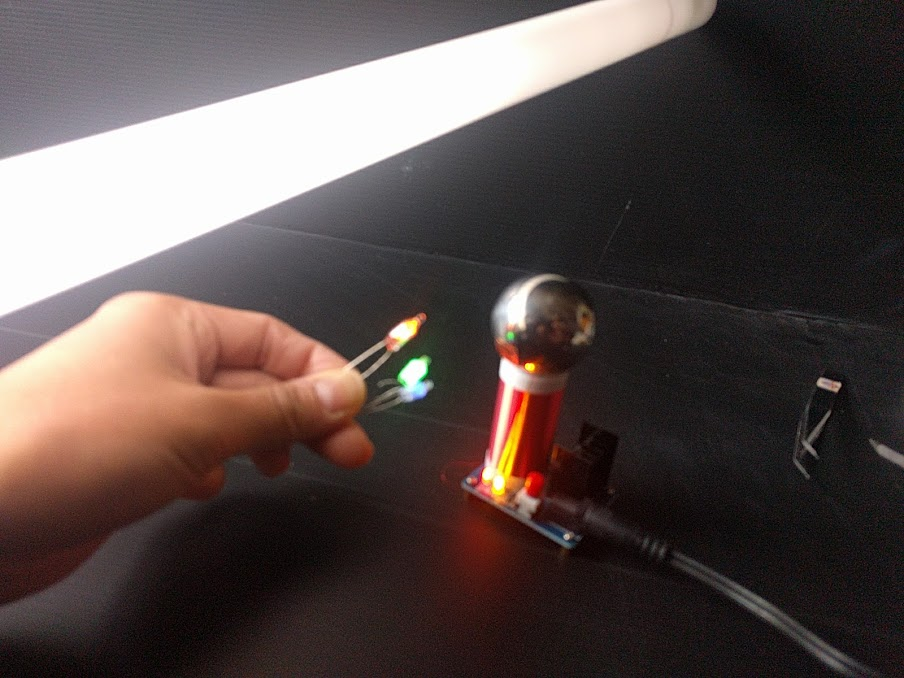
\includegraphics[width=0.5\maxwidth]{./images/c19f0873-8b39-9405-1486-8cfd43e38d78.jpeg}
\caption{ファイル名}
\label{image:qiita2review:c19f0873-8b39-9405-1486-8cfd43e38d78}
\end{reviewimage}

\begin{reviewemlist}
[scale=0.5]![ファイル名](https://qiita{-}image{-}store.s3.amazonaws.com/0/139524/c19f0873{-}8b39{-}9405{-}1486{-}8cfd43e38d78.jpeg)
\end{reviewemlist}

と書けば、Qiita上では大きく、紙媒体に印刷したときには50\%で印刷される。
けれども
[scale=0.5]というのが表示されてしまう。

少し書式を変更。

\begin{reviewemlist}
[]( scale=0.5 )![ファイル名]( https://qiita{-}image{-}store.s3.amazonaws.com/0/139524/c19f0873{-}8b39{-}9405{-}1486{-}8cfd43e38d78.jpeg )
\end{reviewemlist}

とした。

\begin{reviewimage}
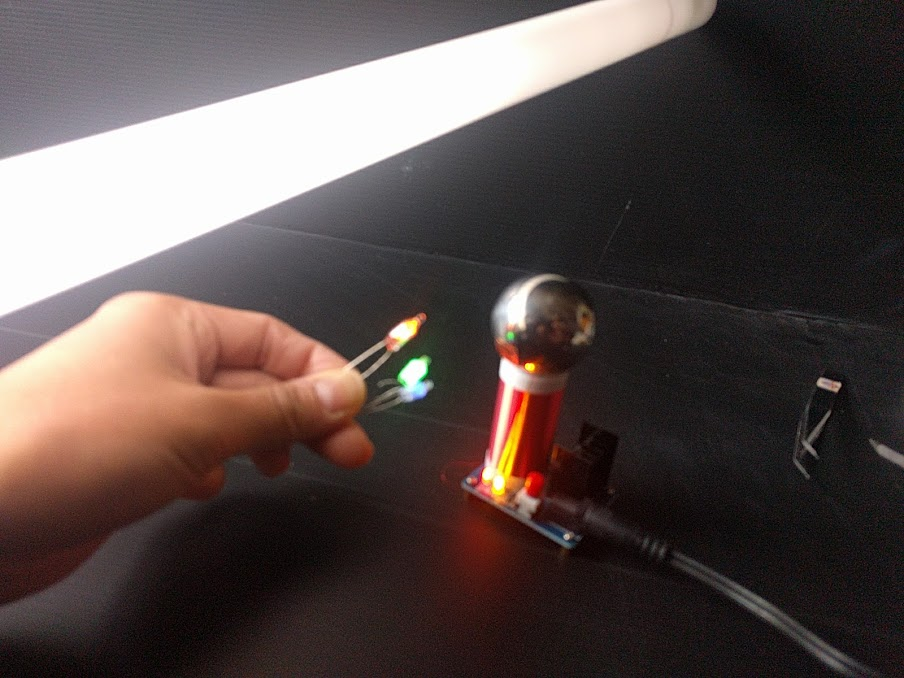
\includegraphics[scale=0.5 ]{./images/c19f0873-8b39-9405-1486-8cfd43e38d78.jpeg}
\caption{ファイル名}
\label{image:qiita2review:c19f0873-8b39-9405-1486-8cfd43e38d78}
\end{reviewimage}

しかしながら md2review でエラーが起こる

\begin{reviewemlist}
 md2review qiita2review2.md
/var/lib/gems/2.3.0/gems/md2review{-}1.11.0/lib/redcarpet/render/review.rb:299:in `remove\textunderscore{}inline\textunderscore{}markups': undefined method `gsub' for nil:NilClass (NoMethodError)
    from /var/lib/gems/2.3.0/gems/md2review{-}1.11.0/lib/redcarpet/render/review.rb:191:in `link'
    from /var/lib/gems/2.3.0/gems/md2review{-}1.11.0/lib/md2review/markdown.rb:13:in `render'
    from /var/lib/gems/2.3.0/gems/md2review{-}1.11.0/lib/md2review/markdown.rb:13:in `render'
    from /var/lib/gems/2.3.0/gems/md2review{-}1.11.0/bin/md2review:54:in `\textless{}top (required)\textgreater{}'
    from /usr/local/bin/md2review:22:in `load'
    from /usr/local/bin/md2review:22:in `\textless{}main\textgreater{}'

\end{reviewemlist}

\begin{reviewemlist}

[]( scale=0.5 )

\end{reviewemlist}

という書き方はmarkdownのコメントアウトなので、これでエラーが起こるとは情けないぞ。

\begin{reviewemlist}
[](
)
\end{reviewemlist}

こんなのでも同様のエラー。
仕方がないので通常のコメントはふつーに消去、\texttt{scale=0.5 )} は \texttt{[scale=0.5]} にするフィルタを作り、md2reviewをかける前に適用するようにしよう。

「preprosess.rb」

\begin{reviewemlist}
\#\#!/usr/bin/env ruby
\#\# this is not support \textdollar{}...\textdollar{} in inline htmltag,link,image.
codeBlock=false
incomment=true
while line = gets
  line.chomp!
  if ( codeBlock == false \&\& md1 = line.match(/\textasciicircum{}```/))
      codeBlock=true
      puts line
  elsif ( codeBlock == true \&\& md1 = line.match(/\textasciicircum{}```/))
      codeBlock=false
      puts line
  elsif ( codeBlock == false \&\& md1 = line.match(/\textasciicircum{}\reviewbackslash{}[\reviewbackslash{}]\reviewbackslash{}(\reviewbackslash{} *(scale=.*)\reviewbackslash{} *\reviewbackslash{})!\reviewbackslash{}[.*\reviewbackslash{}]\reviewbackslash{}(.*\reviewbackslash{})/))
      md2 = line.match(/\textasciicircum{}\reviewbackslash{}[\reviewbackslash{}]\reviewbackslash{}(\reviewbackslash{} *scale=.*\reviewbackslash{} *\reviewbackslash{})(!\reviewbackslash{}[.*\reviewbackslash{}]\reviewbackslash{}(.*\reviewbackslash{}))/)
      print "[" + md1[1] + "]" + md2[1]
  elsif ( codeBlock == false )
    offset=0
    while md1 = line.index("[](",offset) do
      thereistex=false
      if ( md2 = line.match(/\reviewbackslash{}\textdollar{}.*?\reviewbackslash{}\textdollar{}/))
        thereistex=true
      end
      inlinecode="nocode"
      inlinetex="notex"
      for  num in offset..md1{-}1
         ch = line[num]
         if ( ch == "`" \&\& inlinecode=="nocode" )
             inlinecode="starting"
         elsif ( ch != "`" \&\& inlinecode=="starting" )
            inlinecode="incode"
         elsif ( ch == "`" \&\& inlinecode=="incode" )
            inlinecode="ending"
         elsif ( ch != "`" \&\& inlinecode=="ending" )
            inlinecode="nocode"
         elsif ( ch == "\textdollar{}" \&\& inlinecode=="nocode" \&\& inlinetex=="notex" \&\& thereistex==true )
            inlinetex="intex"
         elsif ( ch == "\textdollar{}" \&\& inlinecode=="nocode" \&\& inlinetex=="intex" )
            inlinetex="notex"
         end
         print ch
      end
      offset=md1+4
      num=offset{-}1
      if ( inlinetex!="notex" \textbar{}\textbar{} inlinecode!="nocode")
      else
        incomment=true
        while incomment==true do
          if ( line.length \textless{} num )
            if ( line=gets )
              num=0
            else
              incomment=false
            end
          end
          ch=line[num]

          if ( ch == ")" )
            incomment=false
          end
          num=num+1
          offset=num
        end
      end
    end
    line=line[offset,line.length]
    puts line
  else
    puts line
  end
end

\end{reviewemlist}

制限

汚いコードになってしまったし、

\chapter{Re:VIEW を apache で動かす}
\label{chap:reviewOnApache}

「AWS上にRe:VIEW環境を構築する」
http://qiita.com/nanbuwks/items/da9136f1b6f789aaffcf

からの発展で、Re:VIEW を Web上で動かします。

「組版システムReVIEWでQiitaから同人誌原稿を作る」
http://qiita.com/nanbuwks/items/ad4ed8b7fbda846ba997

この仕組みを使ってQiitaにある記事を薄い本形式のPDFにするようにします。

\section{apache と PHP}
\label{sec:6-1}

apt{-}get install apache2
apt{-}get install libapache2{-}mod{-}php5

\section{DocumentRootにreview環境を展開}
\label{sec:6-2}

cd /var/www/html
review{-}init template
chown {-}R www{-}data:www{-}data *

\section{This account is currently not available.}
\label{sec:6-3}

コマンド実行でエラーが出たので/etc/passwdファイルの

として、www{-}dataでシェルログインできるようにします。

\begin{reviewemlist}
www{-}data:x:33:33:www{-}data:/var/www:/usr/sbin/nologin
\end{reviewemlist}

↓

\begin{reviewemlist}
www{-}data:x:33:33:www{-}data:/var/www:/bin/bash
\end{reviewemlist}

su {-} www{-}data

としてチェック。

・・・としていたのですが、ロケール設定だけの問題だったかも知れません。
現在は、ログオンシェルは /usr/sbin/nologin で運用しています。

\section{review環境を展開します。}
\label{sec:6-4}

review{-}init book

各種フォルダを作ります。

mkdir articles
mkdir template

\section{テンプレートを作ります。}
\label{sec:6-5}

\begin{reviewemlist}
cp book/config.yml template
cd template
vim config.yaml
\end{reviewemlist}

config.yamlを適当に書きます。

書籍タイトル、著者、表紙を作らない、などを指定しておくといいでしょう。

複数人で執筆するので、
Qiitaの1つの記事が1章というようになります。

なのでQiitaの記事は

1人目

\begin{reviewemlist}
\#\# 1人目の1章見出し
内容
\#\#\# 1人目の1{-}2章見出し
内容
\#\# 1人目の2章見出し
内容
\end{reviewemlist}

2人目

\begin{reviewemlist}
\#\# 2人目の1章見出し
内容
\#\#\# 2人目の1{-}2章見出し
内容
\#\# 2人目の2章見出し
内容
\end{reviewemlist}

3人目

\begin{reviewemlist}
・
・
・
\end{reviewemlist}

となりますが、これを

\begin{reviewemlist}
\#\# 1人目のタイトル
1人目の肩書、名前
\#\#\# 1人目の1章見出し
内容
\#\#\#\# 1人目の1{-}2章見出し
内容
\#\#\# 1人目の2章見出し
内容
\#\# 2人目のタイトル
2人目の肩書、名前
\#\#\# 2人目の1章見出し
内容
\#\#\#\# 2人目の1{-}2章見出し
内容
\#\#\# 2人目の2章見出し
内容
\#\# 3人目のタイトル
・
・
・
\end{reviewemlist}

とします。

なので、qiitaから取得したmarkdownは、見出しレベルを変更するスクリプトを通します。

\begin{reviewemlist}
sed "s/\textasciicircum{}\#/\#\#/"  qiita.md
\end{reviewemlist}

とすれば良いことになります。

qiita.mdはqiitaから取得したmarkdownです。qiitaからmarkdownを取得するにはwgetを使います。
こういったものも含めて、処理を行うシェルスクリプトを作ります。

\begin{reviewemlist}
\#\# cat qiitaget.sh
URL=`ruby {-}Ku ../../makeurl.rb`
echo \textdollar{}URL
cd images

wget \textdollar{}URL {-}k {-}H {-}r {-}l 1 {-}nH {-}nd {-}A png,PNG,jpg,JPG,jpeg,JPEG,html  {-}R txt
cd ..

rm qiita.md
wget \textdollar{}URL.md {-}O qiita.md
sed "s/\textasciicircum{}\#/\#\#/"  qiita.md \textbar{} ruby {-}Ku ../../qiitamd.rb \textbar{} ruby {-}Ku ../../texblock.rb \textbar{} ruby {-}Ku ../../texinline.rb   \textgreater{} temp.md
head {-}1 temp.md \textbar{} sed "s/\textasciicircum{}/\#/" \textgreater{} \textdollar{}1.md
ruby  ../../makeauthor.rb  \textgreater{}\textgreater{} \textdollar{}1.md
tail {-}n +2 temp.md \textgreater{}\textgreater{} \textdollar{}1.md
ruby ../../escapeincode.rb \textdollar{}1.md \textbar{} ruby ../../preprocess.rb \textbar{}  md2review \textbar{} ruby {-}Ku ../../scalemd.rb \textgreater{} \textdollar{}1.re
rake pdf
mv book.pdf \textdollar{}1.pdf

\end{reviewemlist}

この、qiitaget.shはPHPからコマンド実行関数で呼び出します。

\begin{reviewemlist}
\#\# cat compile.php
\textless{}html\textgreater{}
\textless{}head\textgreater{}
\textless{}meta charset="UTF{-}8"\textgreater{}
\textless{}title\textgreater{}qiita2review\textless{}/title\textgreater{}
\textless{}style type="text/css"\textgreater{}
body \{
  color: \#000;
  background{-}color: \#ffffff;
\}

pre \{
  padding: 1em;
  color: \#aaffaa;
  background{-}color: \#aaaaaa;
\}
\textless{}/style\textgreater{}
\textless{}/head\textgreater{}
\textless{}body\textgreater{}
\textless{}?php

\textdollar{}sectionName = \textdollar{}\textunderscore{}GET["section"];
?\textgreater{}
\textless{}h1\textgreater{}section \textless{}?php echo \textdollar{}sectionName; ?\textgreater{} compile\textless{}/h1\textgreater{}




\textless{}pre\textgreater{}
\textless{}?php
passthru("export LC\textunderscore{}CTYPE=en\textunderscore{}US.UTF{-}8; export LANG=en\textunderscore{}US.UTF{-}8; cd articles/".\textdollar{}sectionName." ; ../../qiitaget.sh ".\textdollar{}sectionName);


  ?\textgreater{}

\textless{}/pre\textgreater{}

\textless{}form action="\textless{}?php echo "articles/".\textdollar{}sectionName."/".\textdollar{}sectionName; ?\textgreater{}.pdf" METHOD="GET" \textgreater{}
\textless{}input type=submit value="View PDF"\textgreater{}
\textless{}/form\textgreater{}

\textless{}form action="make.php" METHOD="GET" \textgreater{}
\textless{}input type=hidden name=section value=\textless{}?php echo \textdollar{}sectionName; ?\textgreater{}\textgreater{}
\textless{}input type=submit value="return"\textgreater{}


\textless{}/form\textgreater{}
\textless{}/body\textgreater{}
\textless{}/html\textgreater{}

\end{reviewemlist}

他のphpファイル、qiitaget.shから呼び出す各種フィルタスクリプトを作ります。

\begin{reviewemlist}
(省略・・・他記事を参照して下さい)

\end{reviewemlist}

ファイルはwww{-}dataをオーナーにします。

\begin{reviewemlist}
\#\# chown {-}R www{-}data:www{-}data *

\end{reviewemlist}

ファイル一覧です

\begin{reviewemlist}
root@ip{-}172{-}30{-}0{-}222:/var/www/html\# ls {-}alh
total 80K
drwxr{-}xr{-}x 5 www{-}data www{-}data 4.0K Apr  6 14:03 .
drwxr{-}xr{-}x 3 root     root     4.0K Apr  6 13:58 ..
drwxr{-}xr{-}x 4 www{-}data www{-}data 4.0K Apr  6 13:48 articles
drwxr{-}xr{-}x 5 www{-}data www{-}data 4.0K Apr  5 20:07 book
{-}rw{-}r{-}{-}r{-}{-} 1 www{-}data www{-}data  803 Apr  5 03:48 compile.php
{-}rwxr{-}xr{-}x 1 www{-}data www{-}data  680 Apr  6 12:31 escapeincode.rb
{-}rw{-}r{-}{-}r{-}{-} 1 root     root      213 Apr  6 14:03 .htaccess
{-}rw{-}r{-}{-}r{-}{-} 1 www{-}data www{-}data 1.1K Apr  5 05:02 index.php
{-}rw{-}r{-}{-}r{-}{-} 1 www{-}data www{-}data  235 Apr  4 16:19 makeauthor.rb
{-}rw{-}r{-}{-}r{-}{-} 1 www{-}data www{-}data 1.4K Apr  5 20:18 make.php
{-}rw{-}r{-}{-}r{-}{-} 1 www{-}data www{-}data   87 Apr  5 03:28 makeurl.rb
{-}rw{-}r{-}{-}r{-}{-} 1 www{-}data www{-}data 1.2K Apr  5 05:11 new.php
{-}rwxr{-}xr{-}x 1 www{-}data www{-}data 2.0K Apr  5 19:11 preprocess.rb
{-}rwxrwxrwx 1 www{-}data www{-}data  536 Apr  6 12:58 qiitaget.sh
{-}rwxrwxrwx 1 www{-}data www{-}data  458 Apr  3 17:45 qiitamd.rb
{-}rwxrwxrwx 1 www{-}data www{-}data  222 Apr  4 13:41 scalemd.rb
{-}rwxr{-}xr{-}x 1 www{-}data www{-}data 1.4K Apr  6 09:11 slash2braceincode.rb
drwxr{-}xr{-}x 2 www{-}data www{-}data 4.0K Apr  4 18:23 template
{-}rwxrwxrwx 1 www{-}data www{-}data  286 Apr  4 12:20 texblock.rb
{-}rwxr{-}xr{-}x 1 www{-}data www{-}data 1.2K Apr  5 11:18 texinline.rb
\end{reviewemlist}

閲覧系は誰でも見せますが、登録系はbasic認証でアクセス制限をかけます。

\begin{reviewemlist}
\#\# cat .htaccess
\textless{}Files \textasciitilde{} "\textasciicircum{}\reviewbackslash{}.(htaccess\textbar{}htpasswd)\textdollar{}"\textgreater{}
deny from all
\textless{}/Files\textgreater{}
AuthUserFile /var/www/.htpasswd
AuthName "Please enter your ID and password"
AuthType Basic
order deny,allow
\textless{}Files new.php\textgreater{}
require valid{-}user
\textless{}/Files\textgreater{}
\end{reviewemlist}

作成したサイトです

\begin{reviewimage}
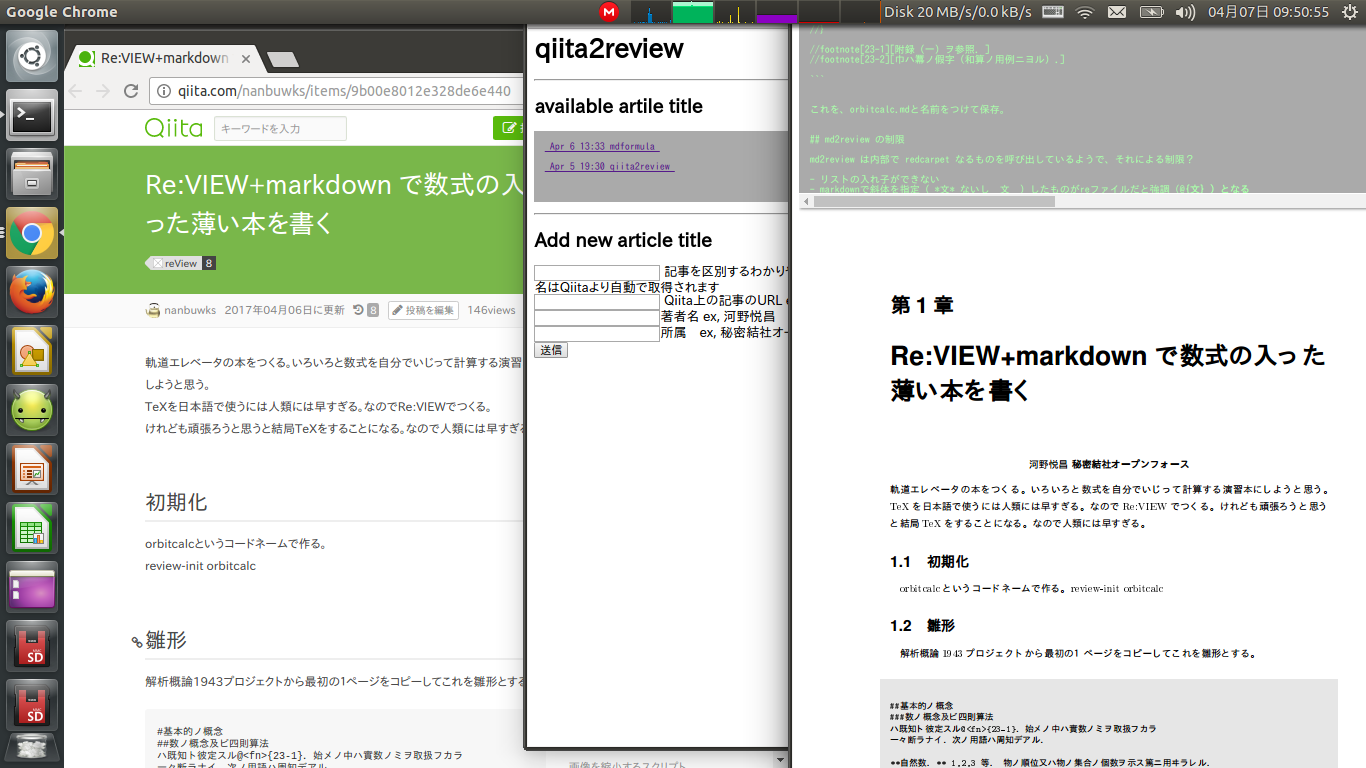
\includegraphics[width=\maxwidth]{./images/7b11276e-74ae-e25a-0872-3726cec353fb.png}
\caption{Screenshot from 2017{-}04{-}07 09{-}50{-}56.png}
\label{image:reviewOnApache:7b11276e-74ae-e25a-0872-3726cec353fb}
\end{reviewimage}


\renewcommand{\chaptermark}[1]{\markboth{\appendixname\thechapter~#1}{}}
\reviewappendix


%% backmatter begins
\backmatter



%%% profile

%%% advfile

%%% colophon
%% okuduke
\reviewcolophon
\thispagestyle{empty}

\vspace*{\fill}

{\noindent\reviewtitlefont\Large Qiita と Re:VIEW を使ってオンラインで記事を寄せあい同人誌を作って 同時にWebコンテンツとして公開できるシステムがこんなに便利なわけはない} \\
\rule[8pt]{14cm}{1pt} \\
{\noindent
2017年4月9日 初版第1刷 発行
}

\begin{tabular}{ll}
著 者 & 日本Androidの会秋葉原支部ロボット部 \\

\end{tabular}
 \\
\rule[0pt]{14cm}{1pt} \\

%%% backcover

\end{document}
